\chapter{A rendelések adatainak nyilvántartása}

Itt magáról az adatmodellről van szó gyakorlatilag. Itt érdemes kifejteni, hogy milyen adat, és hol kerül majd tárolásra. Az ER jellegű diagram, illetve az SQLAlchemy-s modellek egyszerűsített változata kellene majd ide.

A rendelések adatainak nyilvántartása
Az adatbázis tervezése során az egyik fő célom az volt, hogy könnyen módosítható, illetve kibővíthető legyen a rendszer. Első lépésként a fontosabb egyedeket határoztam meg, majd a köztük lévő kapcsolatokat. A dolgozatom készítése során elkészítettem két kezdetleges adatmodellt, amelyeknek az összefésüléséből megszületett a végleges adatmodell. Az alkalmazás implementálása során számos alkalommal kellett módosítanom az adatbázist.

Az általam tervezett adatmodell egyes táblái és a köztük lévő kapcsolatok \aref{fig:rendeles_sema} ábrán láthatók.

\begin{figure}
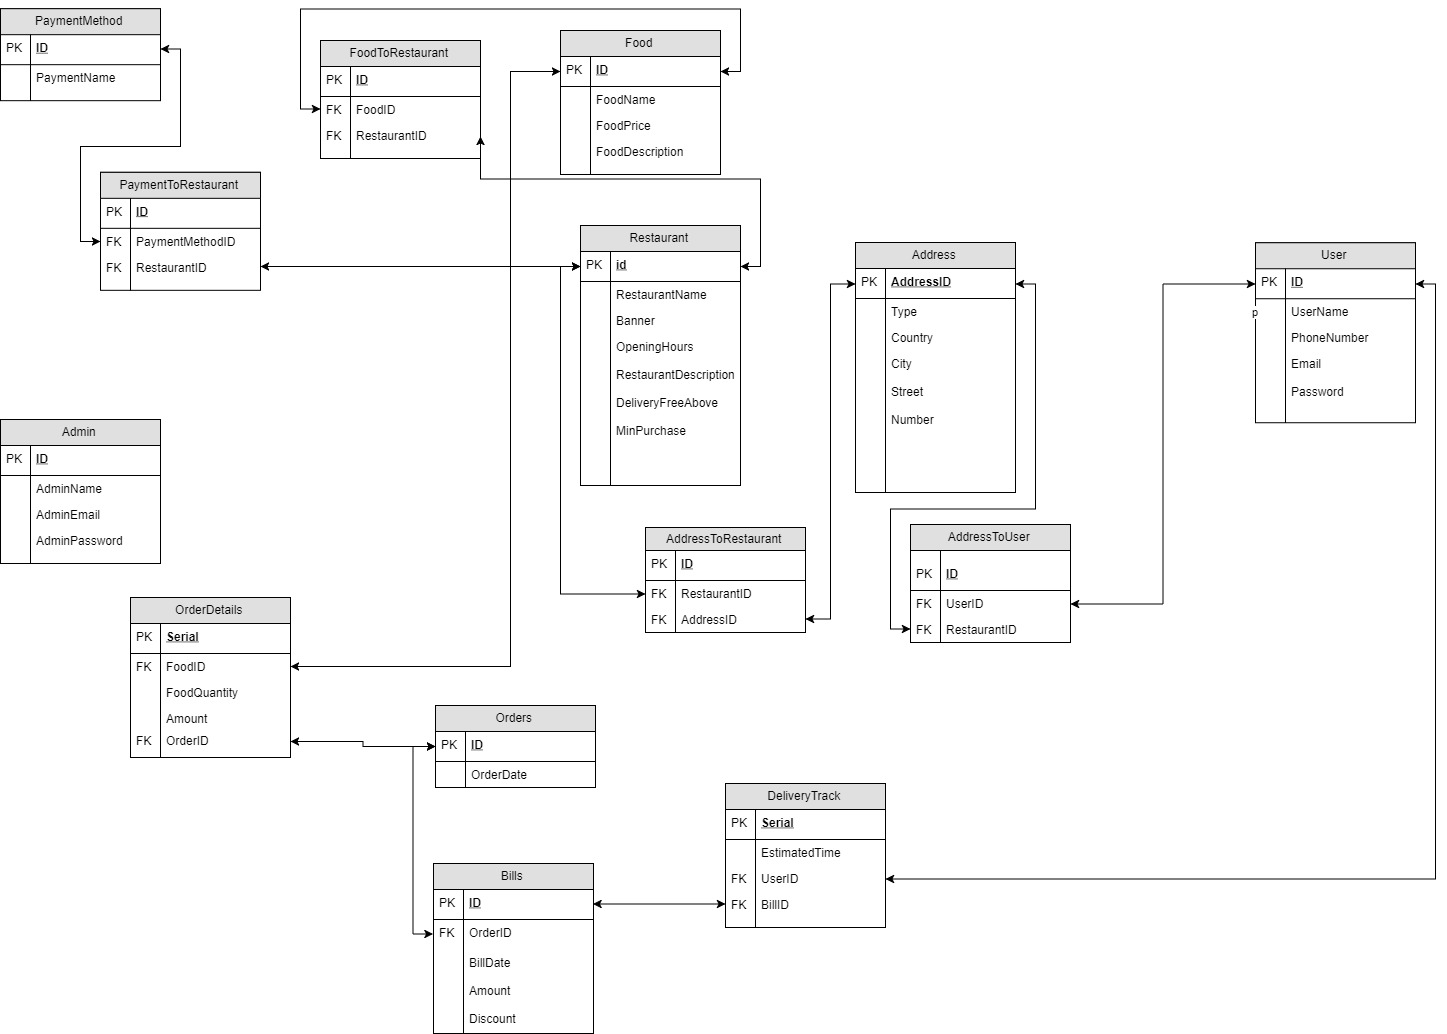
\includegraphics[scale=0.3]{kepek/rendeles_sema.jpg}
\caption{A rendelések adatait kezelő adatábis sémája}
\label{fig:rendeles_sema}
\end{figure}

\section{users}

Az online alkalmazásomon keresztül való étel rendeléshez regisztrált felhasználónak kell lenni. Ez a tábla a regisztrált felhasználókról tartalmaz információkat, illetve az adatbázisban lévő éttermek tulajdonosairól. Minden felhasználó rendelkezik egy azonosítóval, egy kereszt egy vezeték és egy felhasználónévvel, jelszóval továbbá egy telefonszámmal, egy email címmel. Mindegyikhez tartozik egy address, illetve abban az esetben a felhasználó típusa 1-es, - tehát étterem tulajdonos – akkor tartozik hozzá egy restaurant.

\begin{tabular}{|l|l|}
\hline
user\_id & Elsődleges kulcs, a felhasználó azonosítója. \\
first\_name & A regisztrált felhasználó keresztneve. \\
last\_name & A regisztrált felhasználó vezetékneve. \\
user\_name & A regisztrált felhasználó felhasználóneve. \\
password & A felhasználó jelszava. \\
phone\_number & A felhasználó telefonszáma. \\
email & A felhasználó email címe. \\
user\_role & Felhasználó típus, lehetséges értékek: 0: egyszerű felhasználó 1: étterem tulajdonos \\
\hline
\end{tabular}
